%
Le slice rappresentano sequenze di lunghezza variabile di elementi, tutti dello stesso tipo.
Un tipo slice è scritto \verb|[]T|, dove gli elementi sono di tipo \verb|T|: assomiglia ad un array senza una dimensione.

Le matrici e le slice sono intimamente connesse.
Una slice è una struttura dati leggera che dà accesso a una sottosequenza (o anche a tutti) degli elementi di un array, che è noto come \textit{array sottostante} della slice.
Una slice ha tre componenti: un puntatore, una lunghezza e una capacità.
Il puntatore punta al primo elemento dell'array che è raggiungibile attraverso la slice (non necessariamente il primo elemento dell'array).
La lunghezza è il numero di elementi della slice, per cui non può superare la capacità della stessa;
la capacità è di solito il numero di elementi tra l'inizio della slice e la fine dell'array sottostante.
Le funzioni built-in \verb|len| e \verb|cap| restituiscono tali valori.

Più slice possono condividere lo stesso array sottostante e possono riferirsi a parti sovrapposte di esso.
La figura mostra un array di stringhe per i mesi dell'anno e due slice sovrapposte di esso.
L'array è dichiarato come:
\begin{lstlisting}[label={lst:lstlisting3-2.1}]
months := [...]string{1: %*``*\)January%*''*\), /* ... */, 12: %*``*\)December%*''*\)}
\end{lstlisting}
quindi gennaio è \verb|months[1]| e dicembre è \verb|months[12]|.
Si è lasciato fuori dalla dichiarazione l'indice \verb|0| così da inizializzare l'elemento ad esso relativo ad una stringa vuota.

L'\textit{operatore di slice} \verb|s[i:j]|, dove \verb|0|$\le$\verb|i|$\le$\verb|j|$\le$\verb|cap(s)|, crea una nuova slice che si riferisce agli elementi dalla posizione \verb|i| fino alla posizione \verb|j-1| della sequenza \verb|s|, dove \verb|s| può essere una variabile array, un puntatore ad un array o un'altra slice.
La slice risultante ha \verb|j-i| elementi.
Se \verb|i| viene omesso, è come aver inserito \verb|0|, analogamente se \verb|j| viene omesso, è come aver inserito \verb|len(s)|.
Così la slice \verb|months[1:13]| si riferisce all'intera gamma dei mesi validi, così come la slice \verb|months[1:]|;
mentre la slice \verb|months[:]| si riferisce all'intero array (dall'elemento \verb|0| all'elemento \verb|12|).

Un esempio di slice sulla sequenza \verb|months|:
\begin{center}
    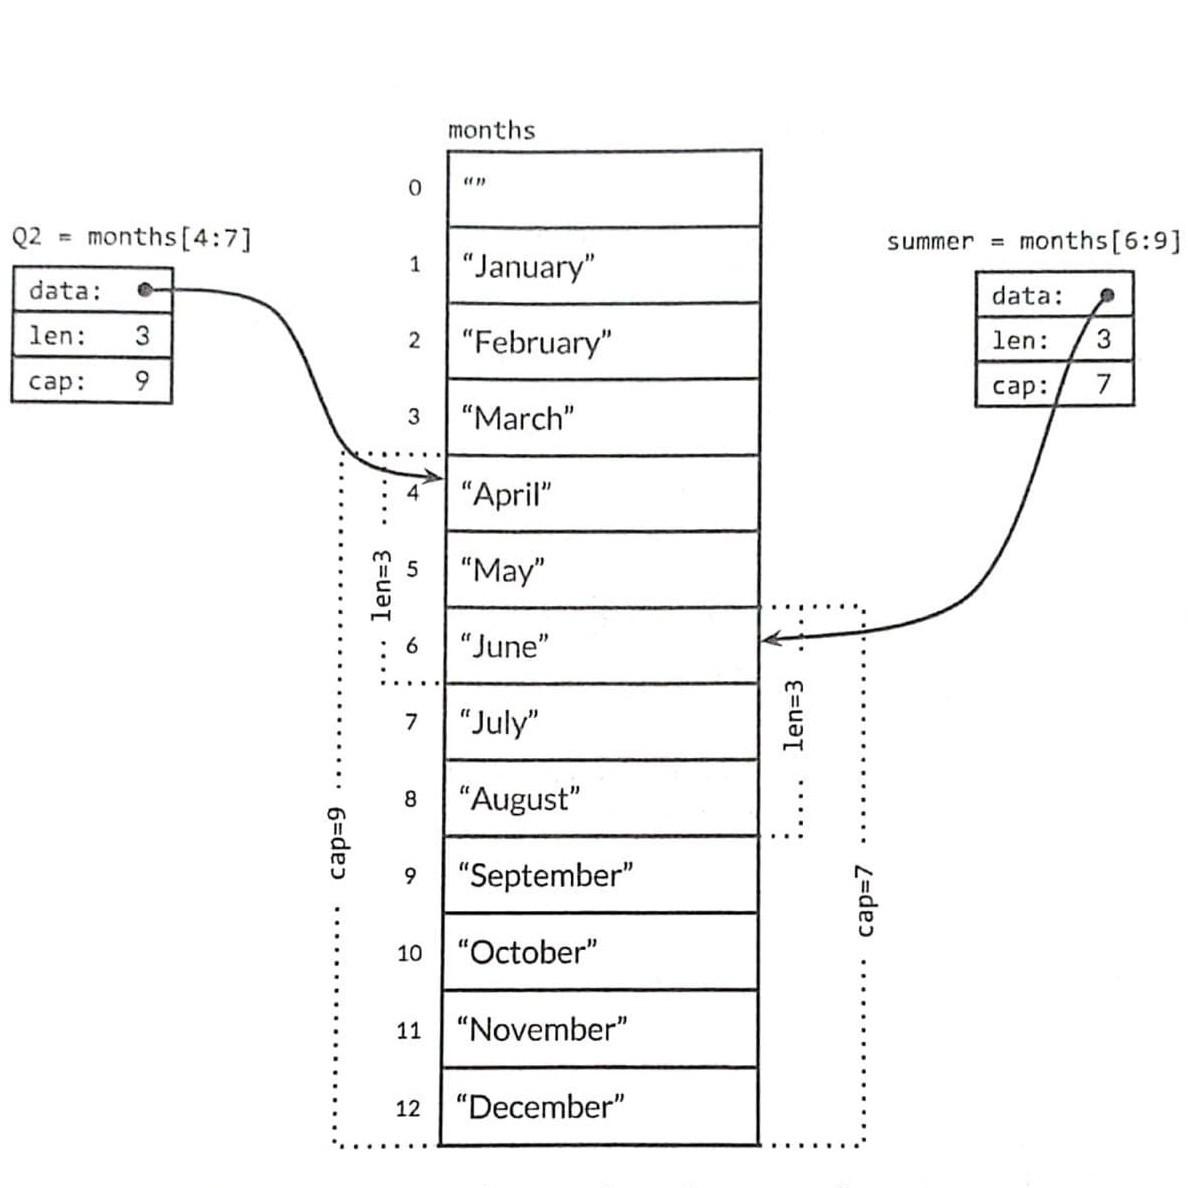
\includegraphics[width=0.5\linewidth]{figures/figura3.1}
\end{center}
\begin{lstlisting}[frame=single, label={lst:lstlisting3-2.2}]
Q2 := months[4:7]
summer := months[6:9]
fmt.Println(Q2)
fmt.Println(summer)
\end{lstlisting}
Output:
\begin{lstlisting}[language=bash, frame=L, label={lst:lstlisting3-2.3}]
[%*``*\)April%*''*\) %*``*\)May%*''*\) %*``*\)June%*''*\)]
[%*``*\)June%*''*\) %*``*\)July%*''*\) %*``*\)August%*''*\)]
\end{lstlisting}
Nell'espressione delle slice, andare oltre \verb|cap(s)| si ottiene una situazione di \verb|panic|, ma andare oltre \verb|len(s)| si ottiene l'estensione della slice, quindi il risultato può diventare più ricco di quello di partenza.
\begin{lstlisting}[frame=single, label={lst:lstlisting3-2.4}]
fmt.Println(summer[:20])    // panic: fuori portata

endlessSummer := summer[:5] // estende una slice entro la sua
                            // capacit%*\textit{à}*\)
fmt.Println(endlessSummer)
\end{lstlisting}
Output:
\begin{lstlisting}[language=bash, frame=L, label={lst:lstlisting3-2.5}]
[June July August September October]
\end{lstlisting}
Poiché una slice contiene un puntatore ad un elemento di un array, passare una slice ad una funzione permette alla funzione di modificare gli elementi dell'array sottostante.
In altre parole, copiare una slice vuol dire creare un \textit{alias} per l'array sottostante.

Uno \textit{slice literal} si presenta come un array literal, una sequenza di valori separati da virgole racchiusi in parentesi graffe, con la dimensione non data.
Questo crea implicitamente una variabile array della giusta dimensione e produce una slice che punta ad essa.
Come con gli array literal, gli slice literal possono specificare in ordine i valori, o assegnare esplicitamente loro gli indici, oppure usare un mix dei due stili.

A differenza degli array, le slice non sono confrontabili, quindi non possiamo usare l'operatore \verb|==| per verificare se due slice contengono gli stessi elementi.
Per i tipi di riferimento come puntatori e channel, l'operatore \verb|==| verifica la \textit{reference identity}, cioè se le due entità riferiscono alla stessa cosa.
La scelta più sicura è quella di non permettere in alcun caso il confronto fra slice.

L'unico confronto legale è con \verb|nil|:
\begin{lstlisting}[frame=single, label={lst:lstlisting3-2.6}]
if summer == nil { /* ... */ }
\end{lstlisting}
Il valore zero di un tipo di slice è \verb|nil|.
Una slice nil non ha un array sottostante.
La slice nil ha lunghezza e capacità zero, ma ci sono anche le slice non nil di lunghezza e capacità zero, come \verb|[]int{}|.
Il valore nil di un particolare tipo di slice può essere scritto usando un'espressione di conversione come \verb|[]int(nil)|.

A meno che non sia chiaramente documentato il contrario, le funzioni Go trattano tutte le slice di lunghezza zero allo stesso modo, sia nil che non nil.

La funzione incorporata \verb|make| crea una slice di un tipo di elemento specificato, e di una certa lunghezza e capacità.
L'argomento capacità può essere omesso, nel qual caso si intende uguale alla lunghezza.
\begin{lstlisting}[frame=single, label={lst:lstlisting3-2.7}]
make([]T, len)
make([]T, len, cap) // uguale a make([]T, cap)[:len]
\end{lstlisting}
La funzione \verb|make| crea una variabile array senza nome e ne restituisce una slice;
l'array è accessibile solo attraverso la slice restituita.
Nella prima forma, la slice è una vista dell'intero array.
Nel secondo, la slice è una vista solo dei primi \verb|len| elementi dell'array, ma la sua capacità include l'intero array.
Gli elementi aggiuntivi sono quindi accantonati per una crescita futura della slice.

La funzione built-in \verb|append| aggiunge elementi alle slice.

Di solito non sappiamo se una determinata chiamata ad \verb|append| causerà una riallocazione, quindi non possiamo supporre che la slice originale punti allo stesso array della slice risultante, né che si riferisca a una diversa.
Allo stesso modo, non dobbiamo presumere che le assegnazioni ad elementi della vecchia slice si rifletteranno (o non si rifletteranno) sulla nuova slice.
Di conseguenza, è normale assegnare il risultato di una chiamata ad \verb|append| alla stessa variabile slice il cui valore è stato passato alla chiamata della funzione \verb|append|:
\begin{lstlisting}[frame=single, label={lst:lstlisting3-2.8}]
var runes []rune
for _, r := range %*``*\)Hello, World%*''*\) {
    runes = append(runes, r)
}
fmt.Printf(%*``*\)%q\n%*''*\), runes)
\end{lstlisting}
Output:
\begin{lstlisting}[language=bash, frame=L, label={lst:lstlisting3-2.9}]
[`H' `e' `l' `l' `o' `,' `W' `o' `r' `l' `d']
\end{lstlisting}
\
Inoltre, la funzione \verb|append| ci permette di aggiungere più di un nuovo elemento, o anche una slice intera dello stesso tipo.
\begin{lstlisting}[frame=single, label={lst:lstlisting3-2.10}]
var x []int
x = append(x, 1)
x = append(x, 2, 3)
x = append(x, 4, 5, 6)
x = append(x, x...) // Aggiunge la slice x
fmt.Println(x)
\end{lstlisting}
Output:
\begin{lstlisting}[language=bash, frame=L, label={lst:lstlisting3-2.11}]
[1 2 3 4 5 6 1 2 3 4 5 6]
\end{lstlisting}
Verrà spiegato più in avanti il perché dell'ellissi ``\verb|...|'' nella chiamata alla funzione \verb|append| nell'ultimo esempio.

Una slice può essere usata per implementare uno stack.
Data uno stack di slice inizialmente vuota, possiamo spingere un nuovo valore alla fine della slice con \verb|append|:
\begin{lstlisting}[frame=single, label={lst:lstlisting3-2.12}]
stack = append(stack, v) // push v
\end{lstlisting}
La testa dello stack è l'ultimo elemento:
\begin{lstlisting}[frame=single, label={lst:lstlisting3-2.13}]
top := stack[len(stack)-1] // top dello stack
\end{lstlisting}
e la restrizione dello stack effettuando il pop dell'elemento:
\begin{lstlisting}[frame=single, label={lst:lstlisting3-2.14}]
stack := stack[:len(stack)-1] // pop
\end{lstlisting}
Per rimuovere un elemento dal centro di una slice, conservando l'ordine degli elementi rimanenti, si usa \verb|copy| per far scorrere gli elementi con il numero più alto verso il basso di uno a riempire lo spazio vuoto generato:
\begin{lstlisting}[frame=single, label={lst:lstlisting3-2.15}]
func remove(slice []int, i int) []int {
    copy(slice[i:], slice[i+1:])
    return slice[:len(slice)-1]
}

func main() {
    s := []int{5, 6, 7, 8, 9}
    fmt.Println(remove(s, 2))
}
\end{lstlisting}
Output:
\begin{lstlisting}[language=bash, frame=L, label={lst:lstlisting3-2.16}]
[5 6 8 9]
\end{lstlisting}